\documentclass[12pt, a4paper, titlepage]{article}
\usepackage{graphicx, amsmath, amsfonts, listings, mathrsfs, color, fancyhdr, geometry, hyperref, amssymb}
\graphicspath{ {images/} }

\geometry{
a4paper,bindingoffset=0.2in,%
            left=1in,right=1in,top=1in,bottom=1in,%
            footskip=.25in
 }
\definecolor{mygreen}{RGB}{28,172,0} % color values Red, Green, Blue
\definecolor{mylilas}{RGB}{170,55,241}
\pagestyle{fancy}
\fancyhf{}
\rhead{Nischal Lal Shrestha}
\lhead{File Handling in C}
\fancyfoot[C]{Page \thepage}
\renewcommand{\headrulewidth}{2pt}

\begin{document}

\begin{titlepage}
	\begin{center}
	{\Large \textbf{Nepal College of Information Technology} \par} 
	{\Large \textbf{ Faculty of Science and Technology} \par} 
	\vspace{0.75cm}
	\begin{center}
		
\includegraphics[scale=0.4]{ncit.png}
	\end{center}
	\vspace{0.75cm}
	{\Large \textbf{Bachelor of Software Engineering} \par}
	\vspace{1.5cm}
	{\scshape\Large Lab Report \par}
	{\huge\bfseries File Handling in C \par}
	\vspace{2cm}

	Candidate name\par
	{\Large \textbf{Nischal Lal Shrestha} \par}
	\vfill
	Supervised by\par
	{\Large \textbf{Asst. P. } \par}
	\vfill
	% Bottom of the page
	{\large \today\par}
	\end{center}
\end{titlepage}

\section{Introduction}

\subsection{What is file?}
File is a collection of bytes that is stored on secondary storage devices like disk. There are two kinds of files in a system.\\
\\
Types of Files
\begin{itemize}
	\item Text files (ASCII)
    \item Binary files
\end{itemize}

\subsection{Basic file operations in C programming}
In C, we can perform four major operations on the file, either text or binary:
\begin{itemize}
	\item Creating a new file
    \item Opening an existing file
    \item Closing a file
    \item Reading from and writing information to a file

\end{itemize}

\section{Working with files}

When working with files, we need to declare a pointer of type file. This declaration is needed for communication between the file and program.
\[
	FILE *fptr;
\]
   
\subsection{Opening a file - for creation and edit} 
Opening a file is performed using the library function in the ``stdio.h" header file: fopen().
The syntax for opening a file in standard I/O is:
\[
ptr = fopen(``fileopen",``mode")
\]

For Example
\[
fopen(``E:\\cprogram\\newprogram.txt","w");
\]

\subsection{Opening Modes in Standard I/O}



\begin{center}
 \begin{tabular}{||c c c||} 
 \hline
 File Mode & Meaning of Mode & During Inexistence of file \\ [0.5ex] 
 \hline\hline
 r & Open for reading & If the file does not exist, fopen() returns NULL. \\ 
 \hline
 w & Open for writing & If the file exists, its contents are overwritten. If the file does not exist, it will be created. \\
 \hline
 a & Open for append & If the file does not exists, it will be created. \\
 \hline
 r+ & Open for both reading and writing & If the file does not exist, fopen() returns NULL.\\
 \hline
 w+ & Open for both reading and writing & If the file exists, its contents are overwritten. If the file does not exist, it will be created.\\ [1ex] 
 \hline
\end{tabular}
\end{center}





\section{Plotting Mathematical Models}
We can use tools like \textbf{Octave} or \textbf{Matlab} to plot various mathematical models. By plotting a mathematical models we can understand the system thoroughly.

\subsection{Plotting Trigonometric Functions}

\lstset{language=Matlab,%
    %basicstyle=\color{red},
    breaklines=true,%
    morekeywords={matlab2tikz},
    keywordstyle=\color{blue},%
    morekeywords=[2]{1}, keywordstyle=[2]{\color{black}},
    identifierstyle=\color{black},%
    stringstyle=\color{mylilas},
    commentstyle=\color{mygreen},%
    showstringspaces=false,%without this there will be a symbol in the places where there is a space
    numbers=left,%
    numberstyle={\tiny \color{black}},% size of the numbers
    numbersep=9pt, % this defines how far the numbers are from the text
    emph=[1]{for,end,break},emphstyle=[1]\color{red}, %some words to emphasise
    %emph=[2]{word1,word2}, emphstyle=[2]{style},    
}

\lstinputlisting{C_Program_To_Add_Item_In_a_File_If_it_doesn't_exist.c}

\begin{figure}[h]
		\centering
		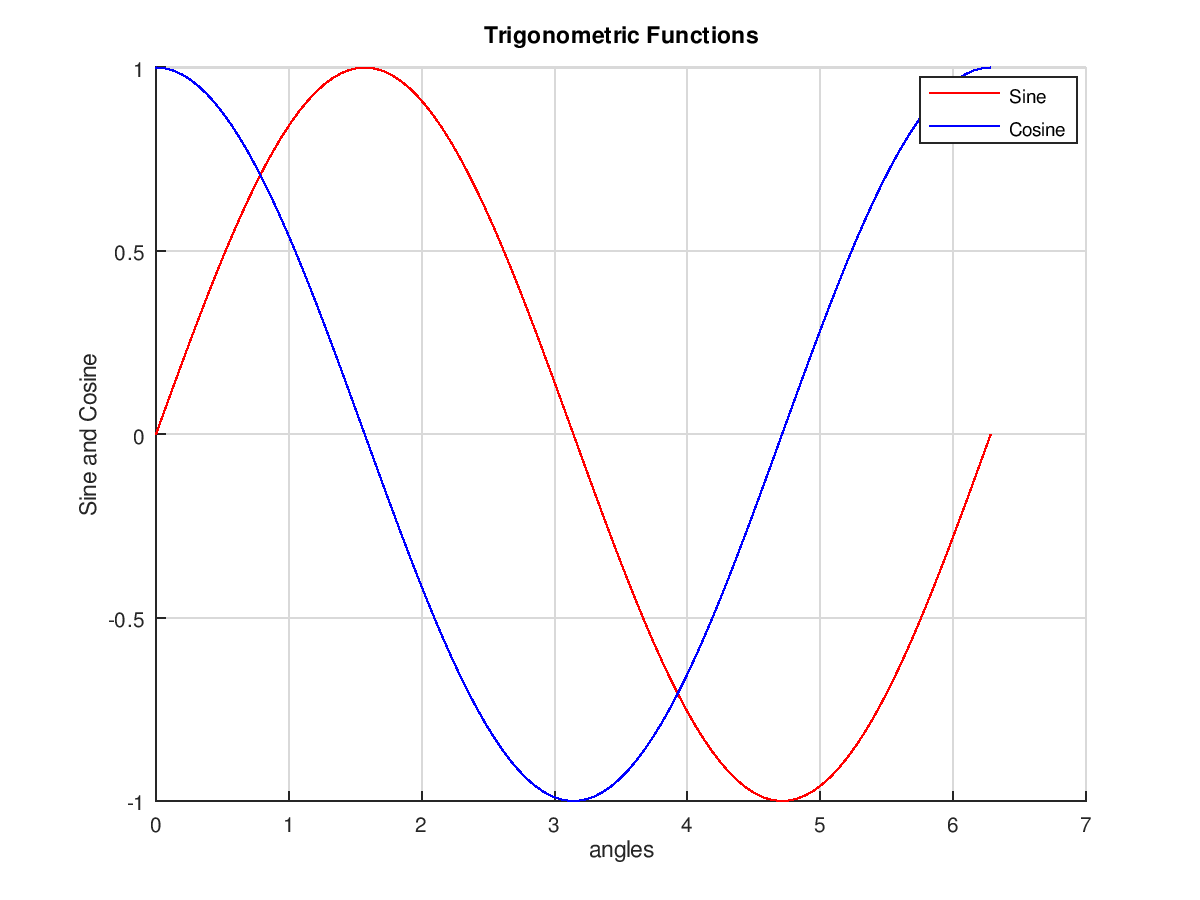
\includegraphics[scale=0.7]{trigonometricFunctionsGraph}
\end{figure}

\subsection{Convergence}
If we suppose $\epsilon$ to be the error quantity of approximated root determined using Newton-Raphson, then by the use of Taylor Series we obtain the following relationship
\[
\epsilon_{n+1} = k \epsilon_n^2
\]
Above equation shows that the error is proportional to the square of the previous error. This means that the number of correct decimal places approximately doubles with each iteration. Such behavior is referred to as \textit{quadratic convergence}.

\section{Algorithm}
An algorithm for the Newton-Raphson Method is obtained simply by using one initial guess as approximated root and by using above generalized formula to calculate the root. \\ \\
The program must also be able to calculate first derivative of the equation provided, which can be done on MATLAB via \verb|diff| command.   An algorithm to solve the non-linear equations using Newton-Raphson Method is defined below:\\
\begin{enumerate}
\item Define $f(x)$, $f'(x)$ and Error ($E$).
\item Input the value of initial root value $x_0$.
\item Caculate
\[
x_1 = x_0 - \frac{f(x_0)}{f'(x_0)}
\]
\item If $(f(x_1) ==  0)$\\
\phantom{x}\hspace{3ex} Display "The root lies at $x =$", $x_0$\\
\phantom{x}\hspace{3ex} Goto Step 6\\
End\\
\item If $(abs(x_1 - x_0) > E)$\\
\phantom{x}\hspace{3ex} Set,\\
\phantom{x}\hspace{6ex} $x_0 = x_1$\\
\phantom{x}\hspace{6ex} $f(x_0) = f(x_1)$\\
\phantom{x}\hspace{6ex} $f'(x_0) = f'(x_1)$\\
\phantom{x}\hspace{3ex} Goto Step 3\\
Else\\	
\phantom{x}\hspace{3ex} Display "The root lies at $x =$", $x_1$\\
End\\
\item Stop
\end{enumerate}
\section{Flowchart}
The flow of the False Position Method program is shown in the figure below
\begin{figure}[h]
		\centering
		
\includegraphics[scale=0.7]{newtonraphsonflowchart}
\end{figure}
\lstset{language=Matlab,
    breaklines=true,
    morekeywords={matlab2tikz},
    morekeywords=[2]{1}, keywordstyle=[2]{\color{black}},
    showstringspaces=false,%without this there will be a symbol in the places where there is a space
    numbers=left,%
    numberstyle={\tiny \color{black}},% size of the numbers
    numbersep=9pt, % this defines how far the numbers are from the text
    emph=[1]{for,end,break},emphstyle=[1]\color{red}, %some words to emphasise
    %emph=[2]{word1,word2}, emphstyle=[2]{style},    
}
\section{Program Code}
The algorithm is implemented on MATLAB and the code is below
\begin{lstlisting}[
    basicstyle=\footnotesize\ttfamily, %or \small or \footnotesize etc.
]
close all;
clear variables;
clc;

func  = input('Enter your desired function:            ');
funcd = input('Enter the derivative of that function   ');
x0    = input('Enter the initial root                  ');

f = inline(func);
fd = inline(funcd);
disp(f);
Error = 0.000005;

fx0 = f(x0);
fdx0 = fd(x0);
x1 = (x0 - (fx0 / fdx0));
fx1 = f(x1);
fdx1 = fd(x1);

if(fx1 == 0)
    result = strcat('The root lies at x = ', num2str(x1));
end

disp('---------------------------------------------------');
disp('      x0       f(x0)     fd(x0)      x1      f(x1)    ');
disp('---------------------------------------------------');
result = [x0, fx0, fdx0, x1, fx1];
disp(result);

while(abs(x1 - x0) > Error)
    x0 = x1;
    fx0 = fx1;
    fdx0 = fdx1;
    x1 = (x0 - (fx0/fdx0));
    fx1 = f(x1);
    result = [x0, fx0, fdx0, x1, fx1];
    disp(result);    
end

disp('---------------------------------------------------');
result = strcat('The root lies at x = ', num2str(x1));
disp(result);  
\end{lstlisting}

\section{Result and Discussion}
The program is run on MATLAB and upon execution the console window displays the result and or solution of the function. One such output for the equation $f(x) = x* sin(x) + 4*cos(x) - 2$ is shown below.\\
\begin{lstlisting}[
    basicstyle=\footnotesize\ttfamily, caption= Output of the Implementation on MATLABS,
]
Enter your desired function:            'x*sin(x)+4*cos(x)-2'
Enter the derivative of that function   'x*cos(x)+sin(x)-4*sin(x)'
Enter the initial root                  1.6

     Inline function:
     f(x) = x*sin(x)+4*cos(x)-2

---------------------------------------------------------
      x0       f(x0)     fd(x0)      x1      f(x1)       
---------------------------------------------------------
    1.6000   -0.5175   -3.0454    1.4301   -0.0230

    1.4301   -0.0230   -2.7698    1.4218   -0.0001

    1.4218   -0.0001   -2.7698    1.4217   -0.0000

    1.4217   -0.0000   -2.7698    1.4217   -0.0000

---------------------------------------------------------
The root lies at x =1.4217
\end{lstlisting}
The program implemented above is not able to calculate first derivative of the function on own, but it rather asks the user to input the first derivative of the function he/she has entered. This can be solved by using a user defined function which is able to differentiate a function, which is beyond the scope of this report. 

\section{Conclusion}
Newton-Raphson Method is perhaps one of the most widely used root-locating formulas. The main advantage of Newton-Raphson method over other methods is that it converges quadratically as we approach the root. Unlike the bisection and false position methods, the Newton-Raphson technique requires only one inital value $x_0$.  \\ \\
However, the convergence of the Newton-Raphson Method is not guranteed. The convergence depends on the nature of the function and on the accuracy of the initial guess. Bad initial guesses can lead to a chaotic series of iterates which may or may not converge at all. So, the only remedy is to have an initial guess that is 'sufficiently' close to the root. 
\begin{thebibliography}{9}
 
\bibitem{einstein} 
E Balagurusamy. 
\textit{Numerical Methods}. 
McGraw Hill Education, 978-0-07-463311-3, 1999.
 
\bibitem{einstein} 
Chapra S.C. and Canale R.P.. 
\textit{Numerical Methods for Engineers, Sixth Edition}. 
McGraw Hill Education, 978-0-07-340106-5, 2010.
\end{thebibliography}



\end{document}